% 2005 年湖南卷文科第 4 题配图：正方体 ABCD-A1B1C1D1 与截面辅助线
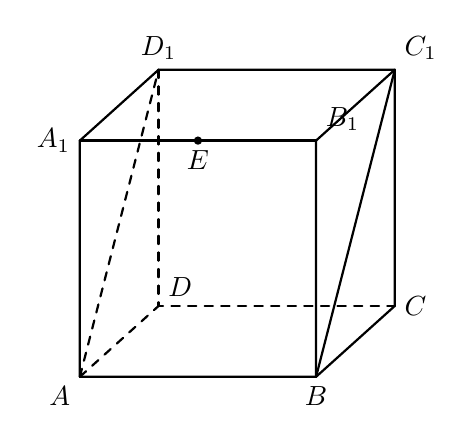
\begin{tikzpicture}[>=latex, line cap=round, line join=round, scale=1.0]
  % 顶点坐标
  \coordinate (A) at (0, 0);
  \coordinate (B) at (3, 0);
  \coordinate (C) at (4, 0.9);
  \coordinate (D) at (1, 0.9);
  
  \coordinate (A1) at (0, 3);
  \coordinate (B1) at (3, 3);
  \coordinate (C1) at (4, 3.9);
  \coordinate (D1) at (1, 3.9);
  
  \coordinate (E) at (1.5, 3);

  % 虚线棱与截面线
  \draw[dashed, thick] (D1) -- (D) -- (C);
  \draw[dashed, thick] (A) -- (D);
  \draw[dashed, thick] (A) -- (D1);

  % 实线棱与截面线
  \draw[thick] (A) -- (B) -- (C) -- (C1) -- (D1) -- (A1) -- cycle;
  \draw[thick] (B) -- (B1) -- (C1);
  \draw[thick] (A1) -- (B1);
  \draw[thick] (B) -- (C1);

  % 点 E
  \fill (E) circle (1.5pt);
  \node[below] at (E) {$E$};

  % 顶点标签
  \node[below left] at (A) {$A$};
  \node[below] at (B) {$B$};
  \node[right] at (C) {$C$};
  \node[above right] at (D) {$D$};
  \node[left] at (A1) {$A_1$};
  \node[above right] at (B1) {$B_1$};
  \node[above right] at (C1) {$C_1$};
  \node[above] at (D1) {$D_1$};
\end{tikzpicture}
